\chapter{Flutter Foundations}
\label{ch:flutter}
In the introduction, a new, promising, cross-platform framework was introduced. The Flutter's primary goal is to provide the ability to build high-performance, high-fidelity apps for \textit{iOS}, \textit{Android}, web, and desktop from a single code-base~\cite{flutter-technical-overview}. In this chapter, the framework's philosophy will be described. Used programming language and theory of reactive programming is briefly introduced. The chapter describes the concept of widgets as a base building block for every application. Later on, one of the most critical topic -- state management is discussed, its existing approaches and which to prefer when building applications. At the end of this chapter, the brief look under the framework's hood is discussed.

Flutter includes a modern react-style framework, a 2D rendering engine, predefined widgets and development tools. The primary premise is a motto "everything is a widget". A widget is an immutable building block of application which is part of the user interface. Each widget can define structural elements such as button, stylistic elements such as colour or it can define the interface's layout, such as padding. Widgets are composed as a tree hierarchy with composing each widget to another. If any event occurs (such as user interaction), the framework can rebuild part of this tree to redraw the screen.  

\begin{figure}[htp]
    \centering
    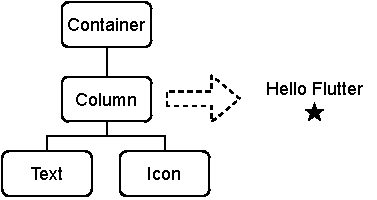
\includegraphics[width=0.5\linewidth]{img/flutter/hello-flutter.pdf}
    \caption{Widget composition example}
    \label{fig:hello-flutter}
\end{figure}

Flutter encourages developers to create and use small, single-purpose widgets and compose them to create complex interfaces and layouts. Take an~example from~\cref{listing:hello-flutter} , where, the root widget, Container is used to create a rectangular visual element. The Container is something like <div> element in HTML.  Under the Container is Column widget which composes children widgets into the vertical direction. Finally, Text widget displaying text "Hello Flutter" and Icon widget showing star icon. The~composition hierarchy along with a~result is shown at~\cref{fig:hello-flutter}.

\begin{listing}[ht]
\begin{minted}{dart}
Container(
    padding: const EdgeInsets.all(5.0),
    child: Column(
      mainAxisAlignment: MainAxisAlignment.center,
      children: [
        Text('Hello Flutter'),
        Icon(Icons.star),
      ],
    ),
),
\end{minted}
\caption{Widget composition code example}
\label{listing:hello-flutter}
\end{listing}
% ----- % ----- % ----- % ----- % ----- % ----- % ----- % ----- % ----- % ----- % ----- % ----- % ----- % ----- %
\section{Technical overview}
Flutter uses programming language Dart (specification v2.0~\cite{dart-specs}) also made by Google and is inspired by languages such as JavaScript. Dart using statically typed system with runtime checks, but like many other languages highly use type inference~\cite{dart-type-system}. Dart can be used from writing simple scripts to full-featured applications. The Dart has flexible compiler technology which can decide running code in different ways, depending on the targeted platform~\cite{dart-platforms}. 

\begin{itemize}
    \item \textbf{Dart Native} -- For programs targeting devices (mobile, desktop, server, and more), Dart Native includes both a Dart VM with \gls{jit} compilation and an~\gls{aot} compiler for producing machine code.
    \item \textbf{Dart Web} -- For programs targeting the web, Dart Web includes both a development time compiler (dartdevc) and a production time compiler (dart2js).
\end{itemize}

\begin{figure}[htp]
    \centering
    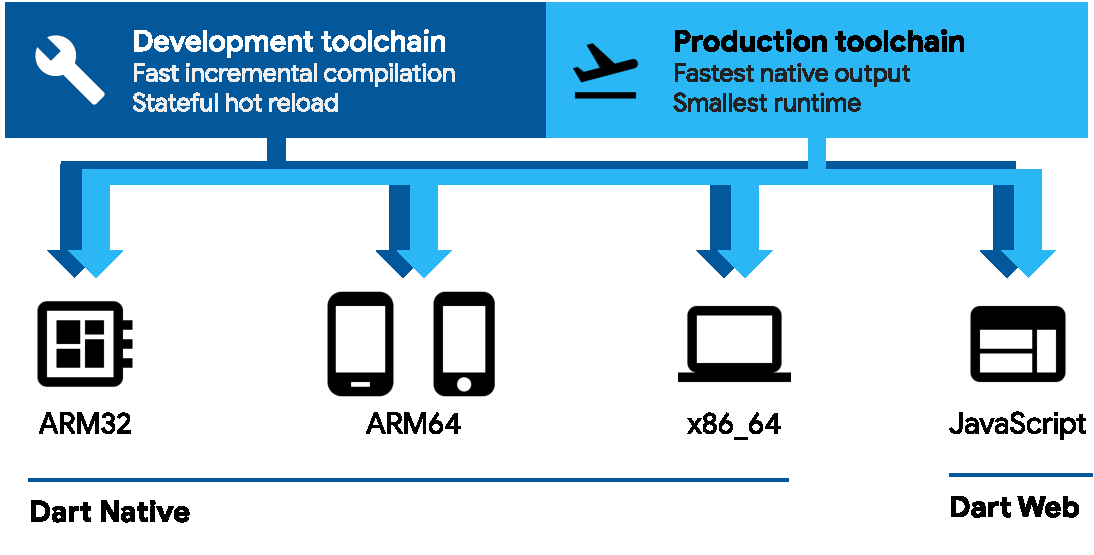
\includegraphics[width=0.8\linewidth]{img/flutter/dart-platforms.pdf}
    \caption{Dart platforms~\cite{dart-platforms}}
    \label{fig:dart-platform}
\end{figure}

Flutter performs the use of both ways. If the targeted platform is web, the \textit{Dart~Web} is used. For other platforms \textit{Dart~Native} is chosen. The Dart~Native's \gls{jit} compilation is highly used to support fast development process with ``hot-reload'' functionality. Then the~\gls{aot} compilation is used for the best-optimised production-ready result on the native platform.  

The Flutter framework is organised into several layers (see~\cref{fig:flutter-layer-cake}), where each layer makes usage of the previous one. The upper layers are more frequently used by developers on a daily basis, and lower layers are used only if the developers need to create particular customisations. 

\begin{figure}[htp]
    \centering
    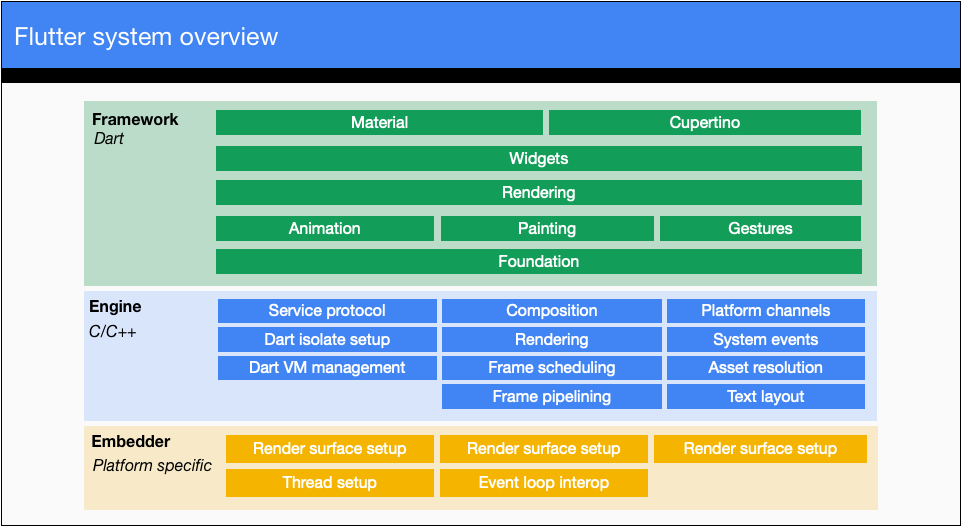
\includegraphics[width=0.8\linewidth]{img/flutter/flutter-layer-cake.png}
    \caption{Flutter system overview~\cite{flutter-technical-overview}}
    \label{fig:flutter-layer-cake}
\end{figure}

Unlike the other frameworks, Flutter uses high-performance 2D rendering engine and draws everything onto the screen directly. That means pixel-perfect control over what and how it is displayed. The most top layer, Material and Cupertino, are set of widgets which defines Material Design (Android systems) and Apple Design component respectively. To highlight that, Flutter does not use native components, but everything draws by himself. These two layers support developers to bring the standardised look and feel to the targeted platform. \todo{review}

% --- # --- # --- # --- # --- # --- # --- # --- # --- # --- # --- # --- # --- # --- # --- # --- # --- # --- #
\subsection{Reactive Programming}
The Flutter makes significant usage from the concept of reactive programming. There is nearly always a~requirement to update data in response to user interaction or any other event such as getting data from the~ server. More than that, sometimes it is necessary to update different parts of the user interface in response to these events. 

The Flutter creates user interface by composing \textbf{immutable} widgets. The immutability is the key point here. Whenever user interface needs to ``redraw'' screen, the~part of the~widget tree is replaced by \textbf{new} widget instances (in fact, it is not simple as that, and this topic is more deeply discussed later in this chapter \todo{remove if not}). In many other \gls{ui} frameworks, such as \textit{Xamarin}, is usually taken the approach of coupling \gls{ui} components with view-models through concepts such as data binding~\cite{xamarin-data-binding}. That means that whenever \gls{ui} needs to~change, the~components mutate application's state. Flutter takes an~entirely different approach. It can be said ``here is the current state of the application, draw something on the screen accordingly''.

\subsubsection{The Notion of Streams}
A Stream can be described as ``a pipe with two ends, only one allowing to insert something into it. When something is inserted into the pipe, it flows inside the pipe and goes out by the other end''~\cite{reactive-didier}. The~Stream can convey any~data type, from simple values to~events, complex object or even another stream. The~data can come to the~Stream, for example, from an external data source such as server connection or from events such as user interactions. In Dart, the Streams support manipulating them, filtering, re-grouping, modify data before they are send and much more. This functionality can be used to build reactive \gls{ui}. The~Flutter has several widgets supporting streams to rebuild part of the~\gls{ui} whenever new data arrived into the~Stream.

The answer to the question ``what is reactive programming`` could be ``Reactive programming is programming with asynchronous data streams``~\cite{reactive-didier},\cite{reactive-red-hat}. Within Flutter framework, anything from an interaction event (tap, gesture), changes on a variable, messages, everything that may change is conveyed and triggered by streams.

That means that with reactive programming, according to~\cite{reactive-didier}, the~application:

\begin{quote}
    \begin{itemize}
        \item becomes asynchronous
        \item is architectured around the notion of Streams and their listeners
        \item when something happens somewhere (an event, a change of a variable) a~notification is sent to a~Stream
        \item if ``somebody'' listens to that Stream, it will be notified and will take appropriate action(s), whatever its location in the~application
    \end{itemize}
    
    From Widgets perspective -- Widget does not longer need to know
    
    \begin{itemize}
        \item what is going to happen next,
        \item who might use this information (no one, one or several Widgets)
        \item where this information might be used (nowhere, same screen, another one, several ones)
        \item when this information might be used (almost directly, after several seconds, never)
    \end{itemize}
\end{quote}

Later on in this chapter, the pattern Business Logic Component (BLoC) is introduced. This pattern uses Streams to manage application life-cycle and state management. 
% ----- % ----- % ----- % ----- % ----- % ----- % ----- % ----- % ----- % ----- % ----- % ----- % ----- % ----- %
\section{Everything Is a Widget}
In this section, we will discuss in more details how the UI is built. Every UI consists of the layout and individual components. The layout defines the screen's base structure, such as a menu on the top and subsequent actions in the bottom. Then the layout is composed of individual components, such as menu, buttons or icons. Together they create a final interface.

These building blocks in the Flutter are called ``Widgets''. Whatever it is simple text, button or complex parts of the~layout, such as grid with multiple columns and rows -- \textbf{everything is a widget}.  Widgets describe what their view should look like given their current configuration and state. When a widget's state changes, the widget rebuilds its description, which the framework diffs against the previous description in order to determine the minimal changes needed in the underlying render tree to transition from one state to the next~\cite{flutter-widget-intro}. As the~composition to the~tree implies, each widget has at most one parent and zero or more children widgets. This tree, called ``widget tree'', is in fact, one of the~three trees involved. The~framework has a sophisticated way of decision about how the~trees should be rebuilt and screen updated. This behaviour is in details described later in this chapter \todo{if not, remove}.

Flutter framework uses only one language to define both the~user interface and business logic as well.  Widgets are Dart class which inherits from some of the widget's base class (typically \textit{StatelessWidget} or \textit{StatefulWidget}). Each widget has a build method which defines how the widget should be built (and drawn on the screen). 
% --- # --- # --- # --- # --- # --- # --- # --- # --- # --- # --- # --- # --- # --- # --- # --- # --- # --- #
\subsection{Widget Are Not Only Visible Parts}
Widgets are not only visible parts of the UI such as clickable buttons, text or icons. The widgets also define layouts such as columns, rows, grids, the margin between other widgets, padding around them and more. 

\begin{figure}[htp]
    \centering
    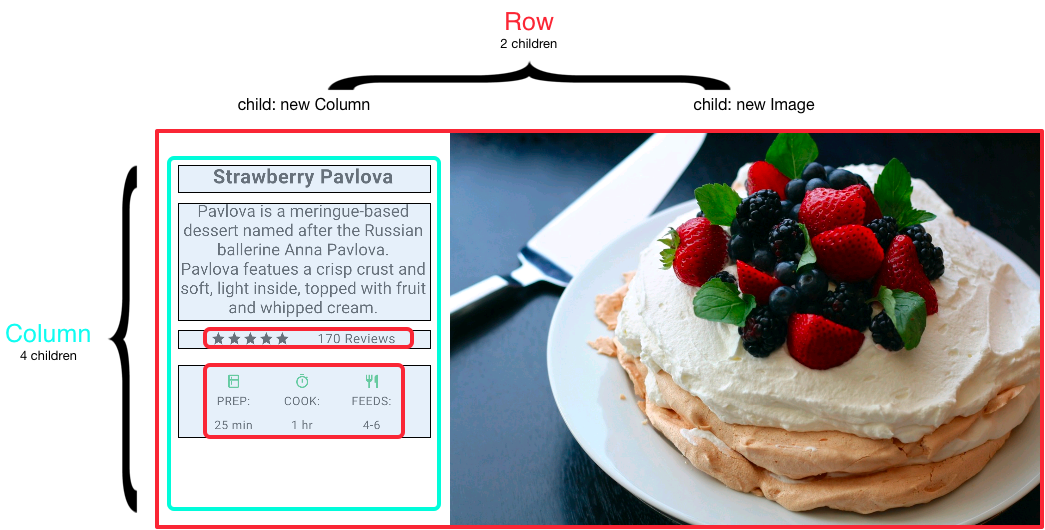
\includegraphics[width=0.75\linewidth]{img/flutter/layout_compose.png}
    \caption{Compose widgets to create layout~\cite{flutter-widget-layout}}
    \label{fig:flutter-compose-widget}
\end{figure}

An example of widget composing creating a layout is shown at~\cref{fig:flutter-compose-widget}. The root widget, a \textit{Row} widget, contains two nested widgets. On the left is a \textit{Column} which contains more nested widgets and on the right, \textit{Image} widget which displays a product image.  The break-down of the left column widget can be seen at~\cref{fig:flutter-compose-widget-detail}. 

\begin{figure}[htp]
    \centering
    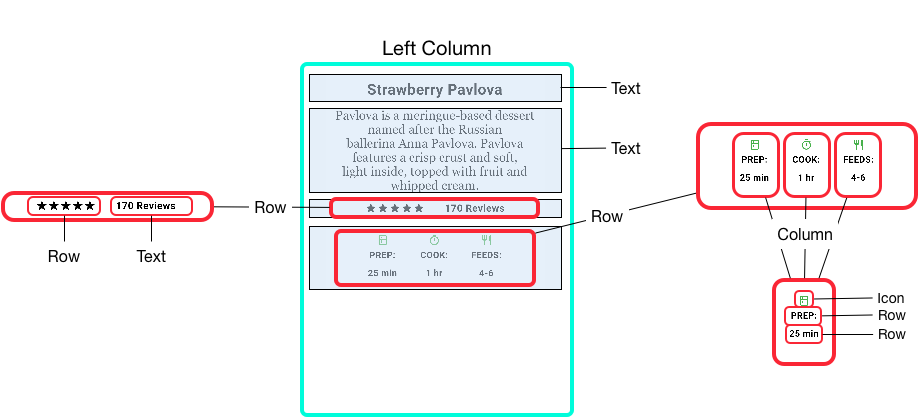
\includegraphics[width=0.75\linewidth]{img/flutter/layout_compose_detail.png}
    \caption{Compose widgets to create layout -- left column detailed~\cite{flutter-widget-layout}}
    \label{fig:flutter-compose-widget-detail}
\end{figure}
% --- # --- # --- # --- # --- # --- # --- # --- # --- # --- # --- # --- # --- # --- # --- # --- # --- # --- #
\subsection{Stateless vs Stateful Widget}
In the introduction was said that Flutter's approach of displaying current user interface is declarative -- ``here is the current state of the application, draw something on the screen accordingly''.  In the Flutter, whenever application' state changes, the user interface is redrawn. There is no imperative changing of the~\gls{ui}, such as \verb|textWidget.text = 'new text'|. The~advantage of the~declarative approach is that there is only one code path for any state of the~\gls{ui}. Developers just describe how the screen should look for a given state, and that is it~\cite{flutter-declarative}. The \gls{ui} can be described as a formula where \gls{ui} is equal to function which takes a state and returns new \gls{ui}~(\cref{fig:flutter-ui-formula}).

\begin{figure}[htp]
    \centering
    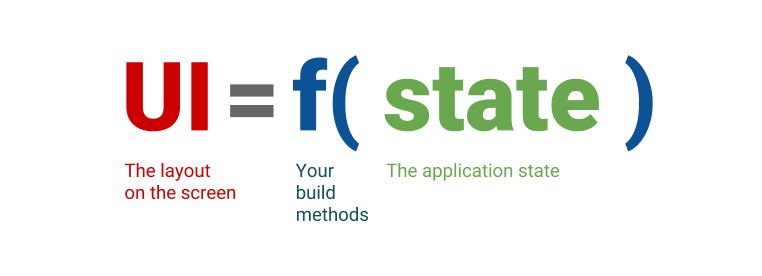
\includegraphics[width=0.6\linewidth]{img/flutter/ui_f_state.png}
    \caption{User interface formula~\cite{flutter-declarative}}
    \label{fig:flutter-ui-formula}
\end{figure}
% --- & --- & --- & --- & --- & --- & --- & --- & --- & --- & --- & --- & --- & --- & --- & --- & --- & --- &
\subsubsection{Build Context}
An~essential part of the widgets is \textit{BuildContext}. A~context is a~reference to the~location of the~widget within the~part of the~tree~\cite{notion-widget-didier}. Each widget has its own context. As~widgets are composed to the~tree, the contexts are as well. The widget has access to its own context and its parent context. 

The \textit{BuildContext} is provided to each widget through the~build method and is used to find the~widget's ancestors.  This is commonly used to obtain a~defined application theme or get a~reference to a~navigator widget, which is used to do navigation between screens. 
% --- & --- & --- & --- & --- & --- & --- & --- & --- & --- & --- & --- & --- & --- & --- & --- & --- & --- &
\subsubsection{Local vs Application State}
The state is anything that forms what should be displayed. The state is any data what are needed in order to rebuild \gls{ui} at the~moment~\cite{flutter-local-app-state}. The~state can be separated into two concepts -- local state and application state. 

\begin{itemize}
    \item \textbf{Local state} -- Local state is which can be tied into one widget. It can be, for example, current tab in the ``tab selector'' widget, current progress of animation or state of checkbox (checked or unchecked).
    \item \textbf{Application state} -- Application State is which can not be local, whenever some information is needed to share across multiple widgets, the~state which should be kept during a~user session. An~example of application state can be a~logged user information, loaded articles from the~server or chat messages.
\end{itemize}
% --- & --- & --- & --- & --- & --- & --- & --- & --- & --- & --- & --- & --- & --- & --- & --- & --- & --- &
\subsubsection{Stateless Widget}
A~Stateless Widget is a widget which does not manage its own state. Once it gets its parameters, and it was built through the build method, it cannot be changed. Remember, that whenever Flutter decides to redraw the~screen, part of the~tree is rebuilt, but with new instances of the~widgets. Typical examples of the Stateless Widgets can be Container, Text or Icon. These widgets accept many parameters which can alter their look (and behaviour), but they cannot be changed later on by~themselves. 
% --- & --- & --- & --- & --- & --- & --- & --- & --- & --- & --- & --- & --- & --- & --- & --- & --- & --- &
\subsubsection{Stateful Widget}
Whenever widget needs to manage its state and for example, for the response of an event wants to mutate its state, the widget should be stateful.  The widget as a~Stateless accepts parameters which can be used to configure this widget but also has an associated object, called state. This state object is an active part of the widget and is used to change widget and force framework rebuilt\gls{ui}.  An~example of a Stateful Widget can be a checkbox with ``checked'' state. 

Stateful Widget does not have only \verb|build| method but has associated State object which defines several methods to support widget's lifecycle. These methods are \verb|initState()| for any state initialisation and \verb|dispose()| to clear any allocated resources. 

The state object is associated with widget's \textit{BuildContext}. This association is permanent, and state object will never change it~\cite{notion-widget-didier}. Even if the~Widget Context can be moved around the~tree structure, the~state will remain associated with that context. This means as a~stateless widget, the~stateful widget itself can be replaced during tree rebuild, but the~state object is persisted. 
% --- & --- & --- & --- & --- & --- & --- & --- & --- & --- & --- & --- & --- & --- & --- & --- & --- & --- &
\subsubsection{Force Rebuild with setState()}
As was stated, Stateful widget can tell the framework to rebuild, and the widget can be redrawn based on changed state. The~stateful widget has method \verb|setState(callback)| which is used to do such rebuild. Inside \verb|callback| developer should change the~widget's state to the~new value and framework will rebuild the widget based on that~new state. 

\subsubsection{Case Study: Counter Application}
Suppose application where are two buttons. One button increments a value (\verb|counter|) and other decrements. The counter value is displayed within two Text widgets located on different places within the application. Whenever any of the buttons are clicked, and the value is changed, all Text widgets should reflect this change.

\begin{figure}[htp]
    \centering
    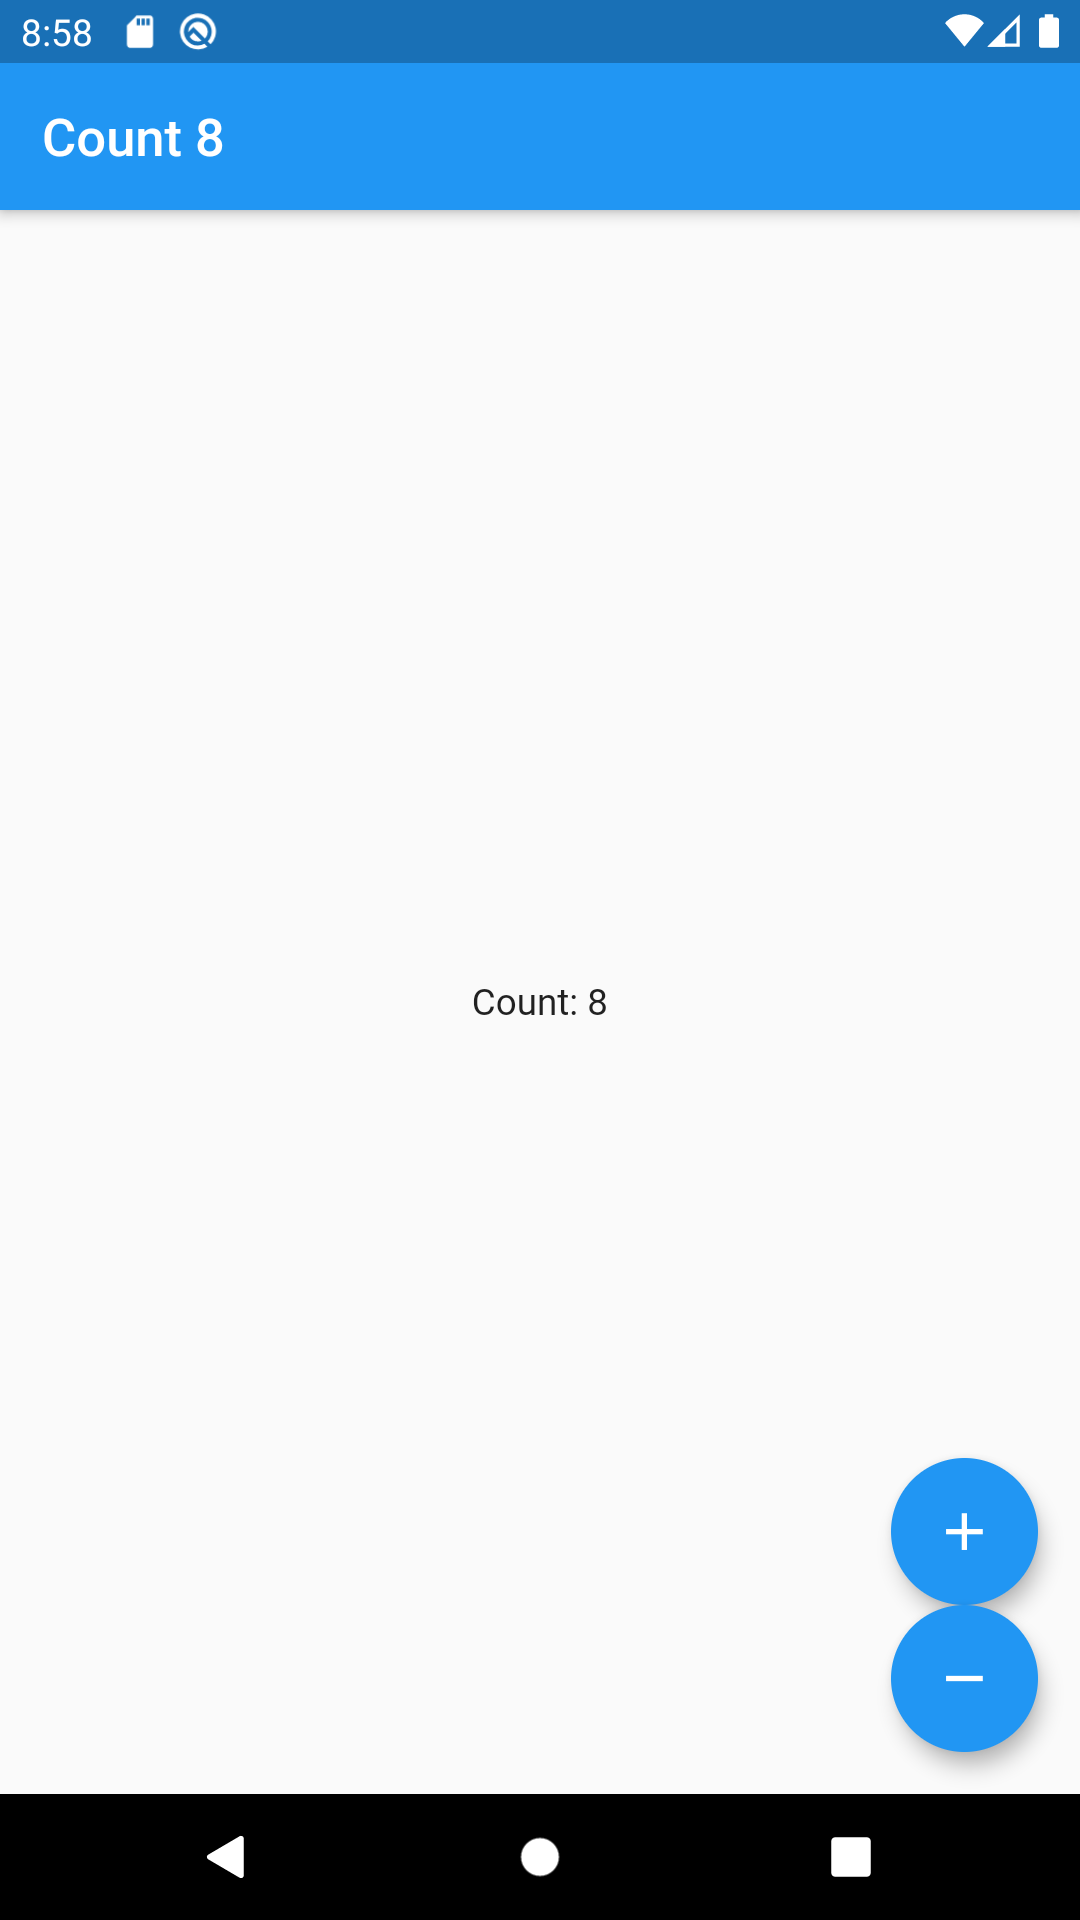
\includegraphics[width=0.33\linewidth]{img/flutter/counter_app_base.png}
    \caption{Counter application}
    \label{fig:counter-app}
\end{figure}

\begin{figure}[htp]
    \centering
    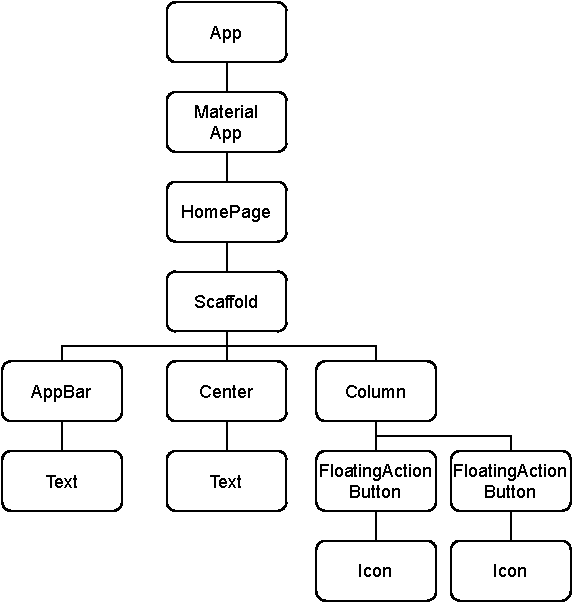
\includegraphics[width=0.40\linewidth]{img/flutter/counter-base.pdf}
    \caption{Counter application widget tree}
    \label{fig:counter-app-widget-tree}
\end{figure}

% \begin{figure}
%     \centering
%     \begin{minipage}{0.3\linewidth}
%         \centering
%         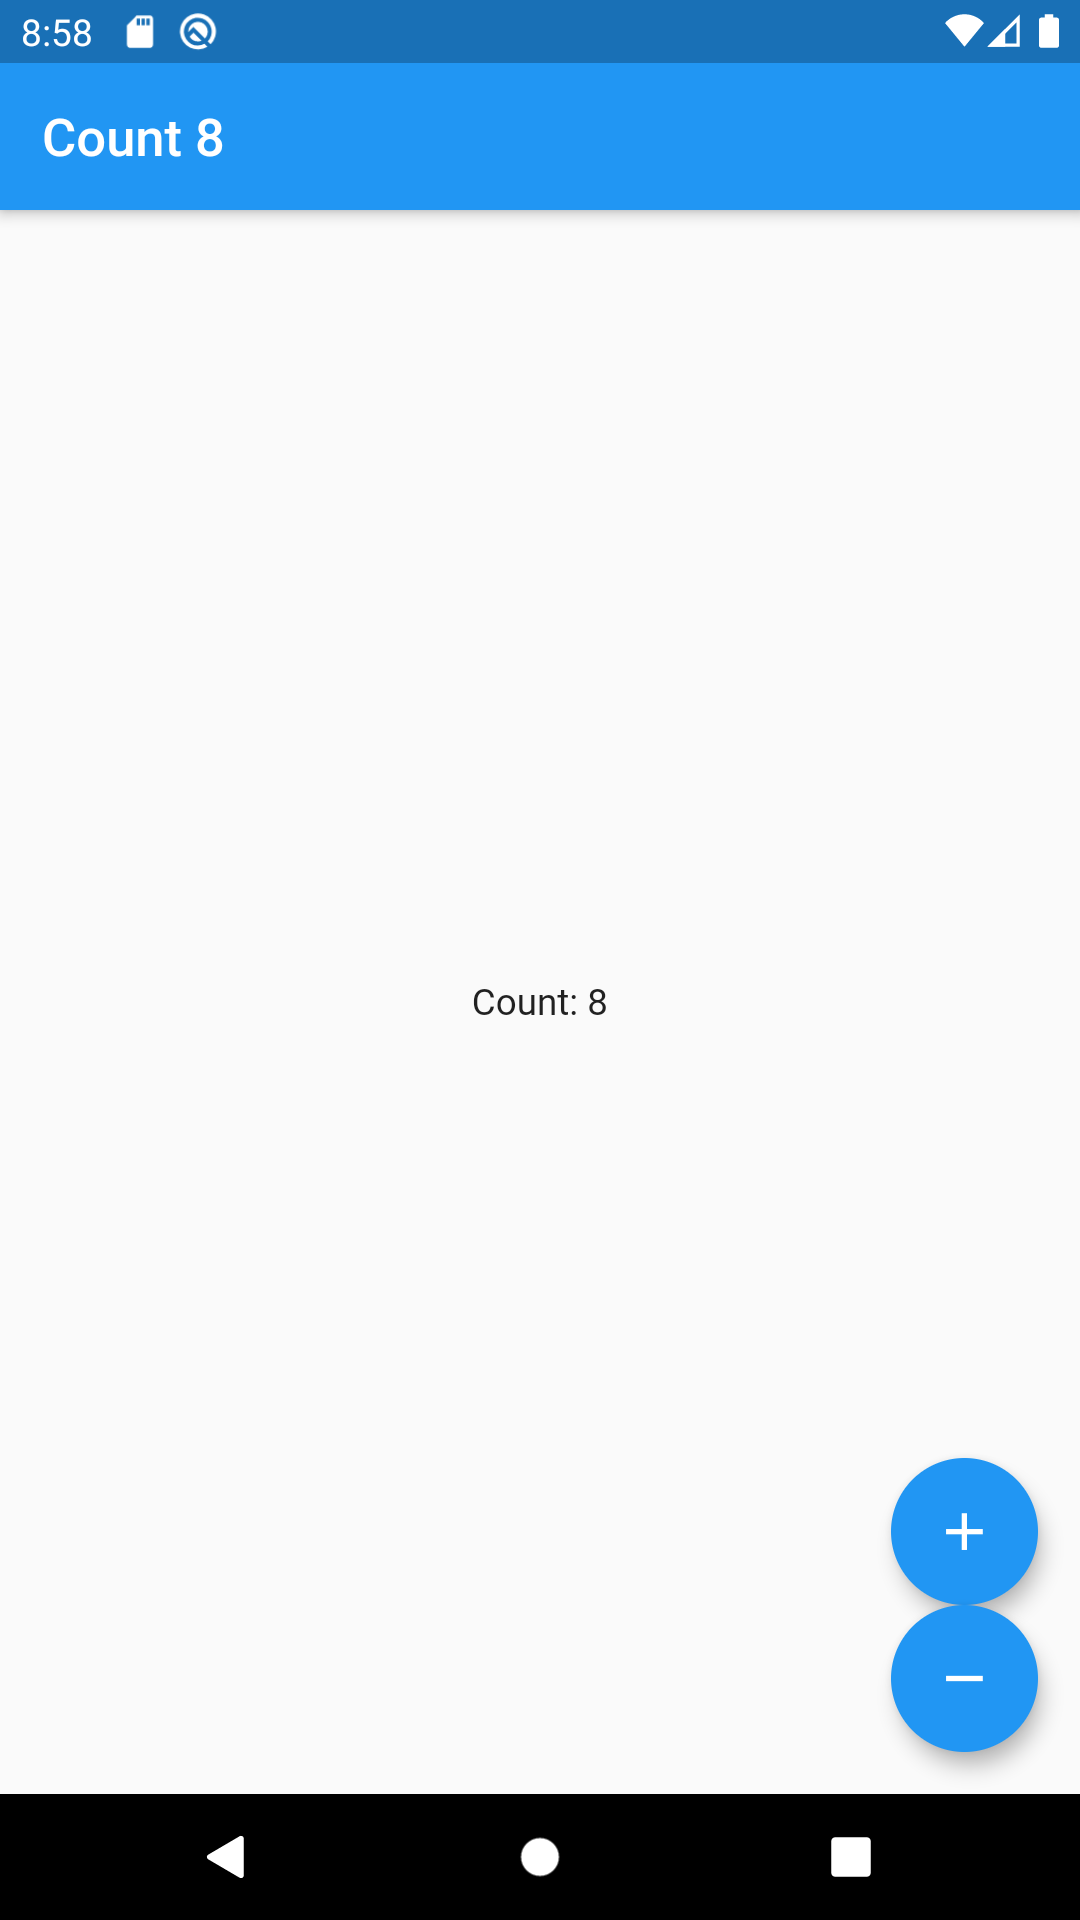
\includegraphics[width=0.40\linewidth]{img/flutter/counter_app_base.png}
%         \caption{Counter application}
%         \label{fig:counter-app}
%     \end{minipage}\hfill
%     \begin{minipage}{0.6\linewidth}
%         \centering
%         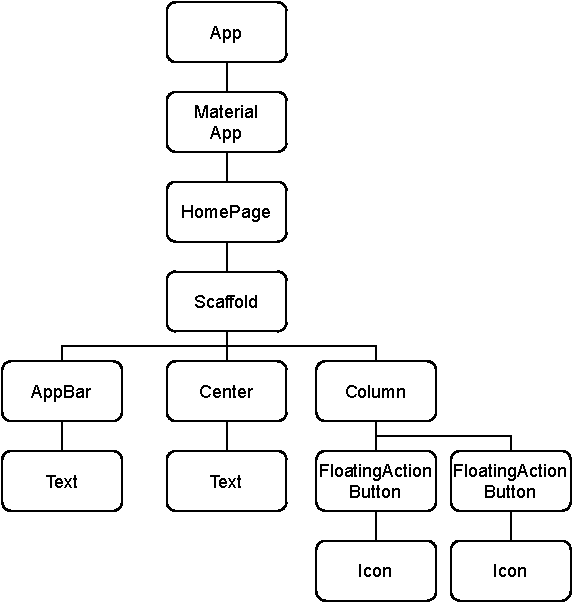
\includegraphics[width=0.40\linewidth]{img/flutter/counter-base.pdf}
%         \caption{Counter application widget tree}
%         \label{fig:counter-app-widget-tree}
%     \end{minipage}
% \end{figure}

Application's layout is shown at~\cref{fig:counter-app} and corresponding widget tree~\cref{fig:counter-app-widget-tree} (shortened for brevity). In the \textit{AppBar} and in the centre of the screen, is \textit{Text} widget which displays current value. On the bottom of the screen are \textit{FloatingActionButtons} widgets, which increments (decrements) counter value. The value needs to be accessible to the Text and to the button as well. Hence, the state is declared within the whole application's widget \textit{HomePage}.  

\begin{listing}[ht]
\begin{minted}{dart}
class HomePage extends StatefulWidget {
  HomePage({Key key}) : super(key: key);
  @override
  _HomePageState createState() => _HomePageState();
}
\end{minted}
\caption{HomePage widget definition}
\label{listing:counter-homepage-widget}
\end{listing}

The~\cref{listing:counter-homepage-widget} shows the definition of the \textit{HomePage} widget. The widget inherits from \verb|StatefulWidget| and declares \textit{HomePageState} which is an associated state object.

\begin{listing}[ht]
\begin{minted}{dart}
class _HomePageState extends State<HomePage> {
  int _counter = 0;

  void _incrementCounter() {
    setState(() {
      _counter++;
    });
  }

  void _decrementCounter() {
    setState(() {
      _counter--;
    });
  }

  @override
  Widget build(BuildContext context) {
    return Scaffold(
      appBar: AppBar(title: Text('Count $_counter')),
      body: Center(child: Text('Count: $_counter')),
      floatingActionButton: Column(
        mainAxisAlignment: MainAxisAlignment.end,
        children: <Widget>[
          FloatingActionButton(
            onPressed: _incrementCounter,
            child: Icon(Icons.add),
          ),
          FloatingActionButton(
            onPressed: _decrementCounter,
            child: Icon(Icons.remove),
          )]));
   }
}
\end{minted}
\caption{HomePageState -- setState example}
\label{listing:counter-base-state}
\end{listing}

\begin{figure}[htp]
    \centering
    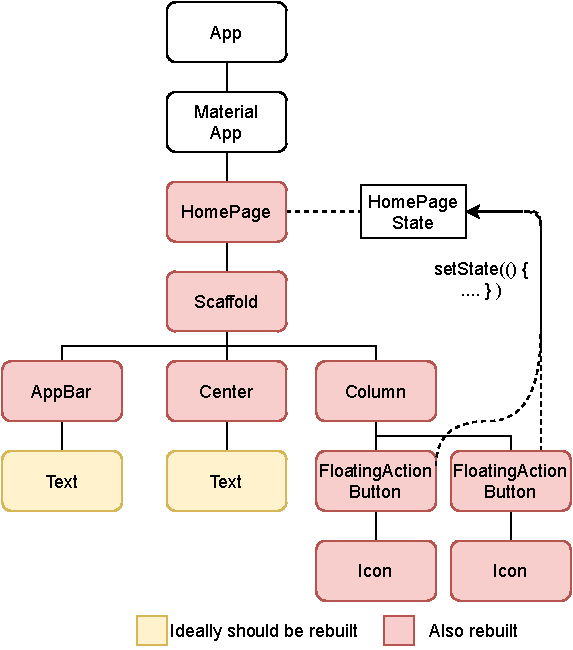
\includegraphics[width=0.40\linewidth]{img/flutter/counter-base-setState.pdf}
    \caption{Expected rebuilt vs actual rebuilt}
    \label{fig:counter-app-base-build}
\end{figure}

The~\cref{listing:counter-base-state} shows definition of \textit{HomePageState}. Notice that \verb|build| method defines \textit{Scaffold} widget as the first widget. Scaffold widget creates the basic layout for Material applications with \textit{AppBar}, body and \textit{FloatingActionButtons}. \textit{HomePageState} defines \verb|int _counter = 0| variable, which is our state. There are also two private methods for incrementing and decrementing counter value. In each method, the \verb|setState()| is called with the appropriate state change.  These two methods are bound to \verb|onPressed| callback within \textit{FloatingActionButton}. 

The expectation is, that if the user pressed any button, the value is increment or decremented respectively. After that part of the~\gls{ui} is rebuild by the framework. This part should be two Text widgets which are interested in counter value. In fact, the state is defined within the~\textit{HomePage} widget, and so, the~whole \textit{HomePage} and its children are rebuilt~(\cref{fig:counter-app-base-build}). In~this small example, it is not really a~problem and performance should not be affected. However, if the~tree is deeply nested with heavy performance widgets (for example animations), it could lead to reduced performant application. 

How to define the application-wide state and prevent the necessary rebuilding part of the widget tree is a subject of ``state management'' section.
% ----- % ----- % ----- % ----- % ----- % ----- % ----- % ----- % ----- % ----- % ----- % ----- % ----- % ----- %
\section{State Management Approaches}
\todo{problem with setState() - define state at the top}
\todo{neccessart rebuilding}
\todo{callback hell}

\todo{inherited widget}

\todo{provider as a wrapper of inherited widget}
\todo{bloc solution}
% ----- % ----- % ----- % ----- % ----- % ----- % ----- % ----- % ----- % ----- % ----- % ----- % ----- % ----- %
\section{Native Features}
\todo{How flutter can use native functions, e.g camera. Flutter plugins.}
% ----- % ----- % ----- % ----- % ----- % ----- % ----- % ----- % ----- % ----- % ----- % ----- % ----- % ----- %
\section{Flutter Internals}
\todo{Flutter canvas engine. Skia framework. How flutter internally works. Widget and widget tree concept. Tree shaking.}
\todo{Usage of Keys to prevent rebuilds}
\todo{How Flutter rebuilds UI -- basic info about Widget Tree, Element Tree, State object, state comparison, const optimization}
\todo{animations? -- good example of rebuilding part of UI}


